
\chapter{Fertigungsüberwachung}\label{Fertigungsueberwachung}
Die Fertigungsüberwachung kontrolliert die Fertigung der Werkstücke und ermöglicht eine Verfolgung der Werkstücke während des Fertigungsprozesses. Dazu nutzt die Fertigungsüberwachung RFID-Lese-/Schreibköpfe die über Profibus mit dem Fertigungsrechner verbunden sind und speichert die ermittelten Timestamps in der im Kapitel \ref{kap:Datenbank} beschriebenen Datenbank ab.
Die Fertigungsüberwachung befindet sich ebenso wie die Datenbank auf dem Fertigungsrechner und ist als Soft-SPS ausgeführt. Für die Programmierung wird CODESYS genutzt. Für den Zugriff auf die Datenbank wird wie in Abschnitt \ref{kap:DatenbankZugriff} ausgeführt das Tool SQL4Automation genutzt.

\section{Konzept}
Das Programm ist so organisiert, das verschiedene Programmteile quasi Parallel ablaufen. Dazu sind die einzelnen Programmteile in Funktionsbausteine ausgelagert. Die Instazen dieser Funktionsbausteine werden in der Main oder in den jeweiligen Instanzen aufgerufen. So lässt sich das Programm Strukturieren. In Abbildung \ref{fig:FB_Uebersicht} ist die Struktur der Funktionsbausteine und deren Instanzen dargestellt. Dabei ist immer der Instanzenname und in Klammern der Name des Funktionsbausteins angegeben. Türkis hinterlegt sind die Stellen wo ein Funktionsbaustein global instanziert wurde und innerhalb der lokalen Instanz genutzt wird.
\begin{figure}[h]
	    \centering
	    \includegraphics[width=0.7\linewidth]{Bilder/FB_Uebersicht_final.png}
        \caption{Übersicht über die Funktionsbausteine und ihre Instanzen}
        \label{fig:FB_Uebersicht}
\end{figure}
Nähere Informationen zu den einzelnen Funktionsbausteinen sind in Abschnitt \ref{kap:FBs} zu finden. Innerhalb der Funktionsbausteine ist das Programm überwiegend durch Zustandsautomaten organisiert. Dies ermöglicht ein Strukturiertes Programm und den grafischen Entwurf mithilfe eines UML-Zustandsdiagramms.

Aufgeteilt ist das Programm in drei Funktionsteile. Der eine Teil sorgt für das Auslesen und Beschreiben der RFID-Tags. Dabei wird einerseits ein Abbild der aktuell Eingelesenen Werte der RFID-Tags unter den Lesegeräten der Stationen 2 bis 8 erstellt und andererseits der Station 1 der Wert zugewiesen mit der der nächste RFID-Tag beschrieben werden soll. Dieser Teil befindet sich in den Funktionsbausteinen \glqq Aufruf\_RFID\_Channel\_2\_bis\_8\_Lesen\grqq  und \glqq Aufruf\_RFID\_Channel\_1\_Schreiben\grqq . Der zweite Teile sorgt für die Kommunikation zwischen der Soft-SPS und der Datenbank und befindet sich im global instanzierten Funktionsbaustein \glqq Datenbank\_Read\_Write\grqq . Der letzte Teil sorgt für die Kommunikation zwischen den beiden anderen Teilen. Die eingelesenen Werte der RFID-Lesegeräte und die aus Datenbankabfragen gewonnen Werte werden ausgewertet und daraus Anweisungen an die anderen Programmteile generiert. 

\section{Funktionsbausteine}\label{kap:FBs}

\subsection{FB Aufruf\_RFID\_Channel\_2\_bis\_8\_Lesen} \label{kap:FB_Lesen}
Dieser Funktionsbaustein ließt die RFID-Leseköpfe an den Stationen 2 bis 8 aus. Es handelt sich hierbei um eine Erweiterung des im Staterkit zurverfügunggestellten Funktionsbausteins \glqq Aufruf\_RFID\_Channel\_1\_bis\_8\grqq . Die Leseköpfe 2 bis 8 werden nur lesend betrieben. Der eigentliche Zugriff auf die RFID-Leseköpfe findet in den sieben Instanzen des auch mit dem Staterkit zurverfügunggestellten Funktionsbausteins \glqq FB\_RFID\_SS15\grqq  statt. Auch die Initialisierung findet in diesen Instanzen statt und muss über die entsprechende Eingangsvariable gestartet werden .

Die Instanzen des Funktionsbausteins \glqq FB\_RFID\_SS15\grqq  werden in jedem Zyklus aufgerufen. Zu beginn des Funktionsbausteins befindet sich ein Zustandsautomat, der die Initialisierung der Instanzen des  \glqq FB\_RFID\_SS15\grqq  durchführt und den Lesebetrieb festlegt. Um den Code kürzer und Übersichtlicher zu gestalten befindet sich der Zustandsautomat in einer for-Schleife, wobei jeder Schleifendurchlauf einem Lesekopf entspricht. Die entsprechenden Variablen für die Initialisierung befinden sich dazu in einem Array. Der Zustandsautomat für die Initialisierung ist in Abbildung \ref{fig:init_Leseköpfe} dargestellt.

\begin{figure}[h]
	    \centering
	    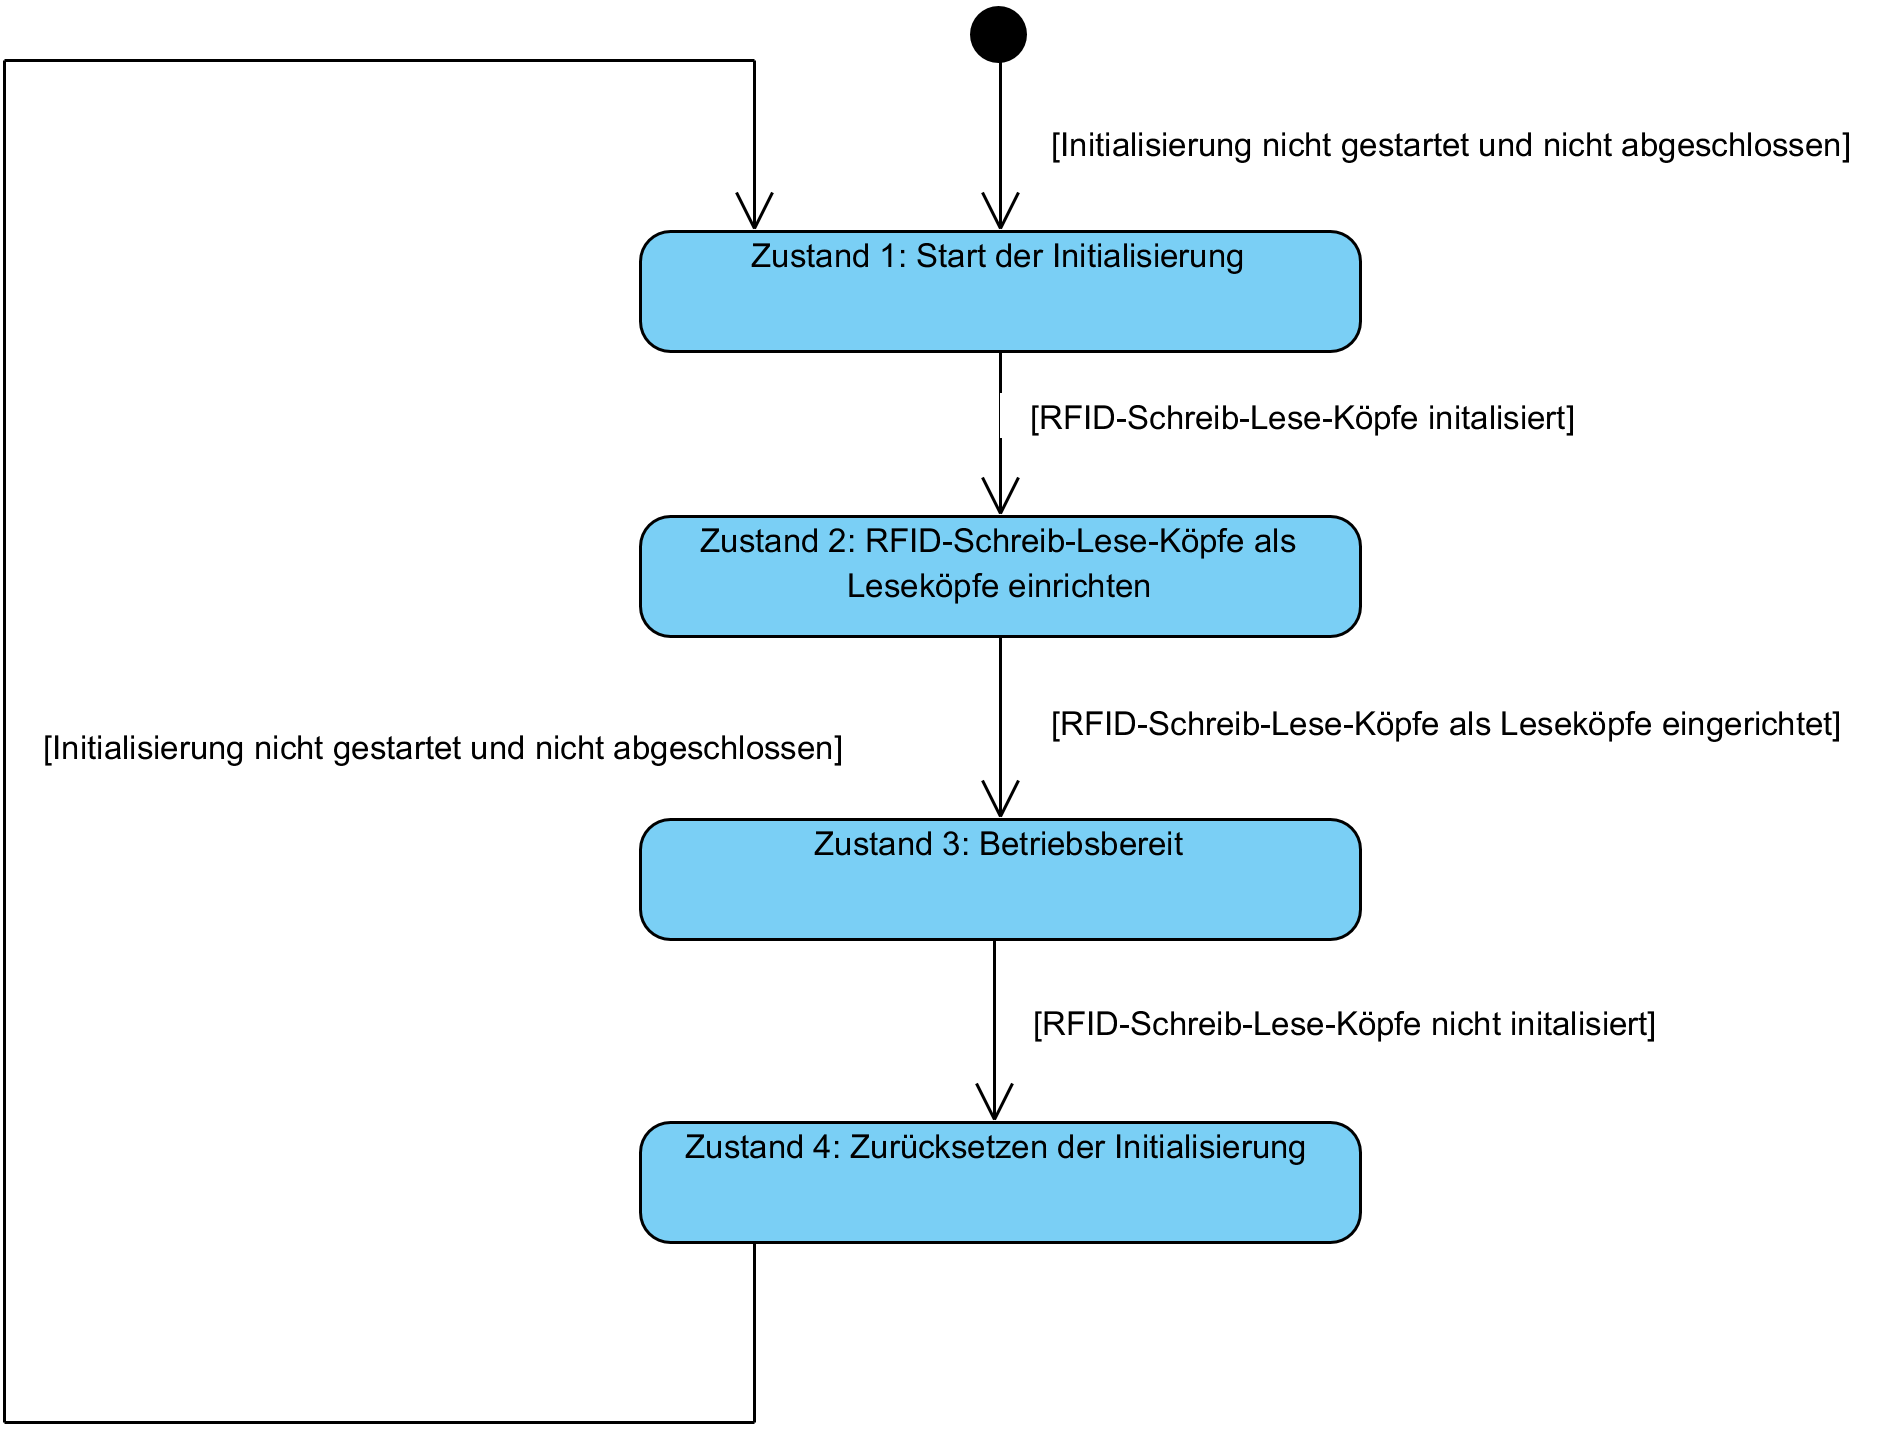
\includegraphics[width=0.7\linewidth]{Bilder/Zustandsdiagramme/RFID_lesen.png}
        \caption{UML-Zustandsdiagramm der Initilisierung der RFID-Leseköpfe 2 bis 8}
        \label{fig:init_Leseköpfe}
\end{figure}

Ist die Initalisierung abgeschlossen werden die RFID-Leseköpfe kontinuierlich ausgelesen. Ist ein RFID-Tag unter dem Lesegerät wird der Wert des Tags in einem Array gespeichert. Dabei entspricht die Stelle im Array der Station, wo der Tag eingelesen wurde. Ist kein Werkstück unter dem RFID-Lesegerät wird in das Array eine 0 geschrieben. Da der Wert den die RFID-Lesegeräte zurückliefern immer dem des zuletzt eingelesenen RFID-Tags entspricht wird mithilfe des Parameters TFR überprüft ob aktuell ein RFID-Tag unter dem Lesegerät ist. Der TFR-Parameter gibt an ob sich ein RFID-Tag innerhalb des Lesebereichs des RFID-Lesekopf befindet. Befindet sich kein RFDI-Tag unter dem Lesekopf wird der Wert auf 0 gesetzt. Befindet sich ein RFID-Tag unter dem Lesegerät wird gewartet bis der Lesekopf den RFID-Tag ausgelesen hat und der Wert ins Array geschrieben. 

Da der RFID-Tag als einzelne Bytes ausgelesen wird müssen diese noch in einen Integer-Wert umgerechnet werden. Dies übernimt die selbstgeschriebene Funktion ByteToInt(), die als Eingangsvariable ein Byte-Array und als Ausgangsvariable einen Integervariable hat.
\subsection{FB Aufruf\_RFID\_Channel\_1\_Schreiben}
Dieser Funktionsbaustein organisiert das beschreiben der RFID-Tags an Station 1. Im Aufbau ist er dem in Abschnitt \ref{kap:FB_Lesen} beschriebenen Funktionsbasutein ähnlich. Allerdings befindet sich hier nur eine Instanz des Funktionsbausteins \glqq FB\_RFID\_SS15\grqq . Der Zustandsautomat entspricht dem in Abbildung \ref{fig:init_Leseköpfe}. Lediglich in Zustand 2 wird der RFID-Lese-/Schreibkopf nicht als Lesekopf sondern als Schreibkopf eingerichtet. 

Über die Rückgabewerte Busy und Done wird detektiert wenn ein RFID-Tag neu beschrieben wurde. Wird ein Schreibvorgang erkannt wird die Globale Variable \glqq WRITE\_RFDI\_DONE\grqq gesetzt. Diese Variable wird im Funktionsbaustein \glqq Timestamp\_anlegen\grqq aus Abschnitt \ref{kap:FB_Timestamp} beim Suchen nach eine neuen Werkstück verwendet. Dort wird sie auch zurückgesetzt. Damit sie nach dem Zurücksetzen nicht sofort wieder gesetzt wird, sollte sich das Werkstück noch unter dem Schreibkopf befinden wird mittels eines Timers \SI{6}{\second} gewartet. Das bedeutet das auch nur alle  \SI{6}{\second} ein Werkstück aus dem Lager geholt werden kann. Diese Zeit wird durch die Roboter allerdings immer weit überschritten.

\subsection{FB FB\_RFID\_SS15}
Der Funktionsbaustein\glqq FB\_RFID\_SS15\grqq wurde mit dem Starterkit zurverfügung gestellt. Der im Programm verwendete Funktionsbaustein entspricht fast kommplet dem Funktionsbaustein aus dem Starterkit weshalb er hier nicht weiter erläutert wird. Nur für das Errorhandling sind wenige Zeilen Code hinzugekommen. 

Ist der Rückgabewert "`Channel\_X\_ERROR"´ wird ein Reset durchgeführt bis der der Fehler behoben wurde. Zum Testen der Fehleranfälligkeit befindet sich ein Zähler im Errorhandling. 

\subsection{FB Werkstueck\_Tagen}
Immer wenn ein Roboter ein Werkstück aus dem Lager holen soll wird von der Fertigungsplanung in die Datenbank geschrieben um welches Werkstück es sich handelt. Dieser Funktionsbaustein fragt durchgehend die Datenbank ab und ermittelt so welches die nächste Id ist die an Station 10 auf den RFID-Tag des Werkstücks geschrieben werden muss. In Abbildung \ref{fig:FB_Werkstueck_taggen} ist das dazugehörige Zustandsdiagramm dargestellt.
\begin{figure}[h]
	    \centering
	    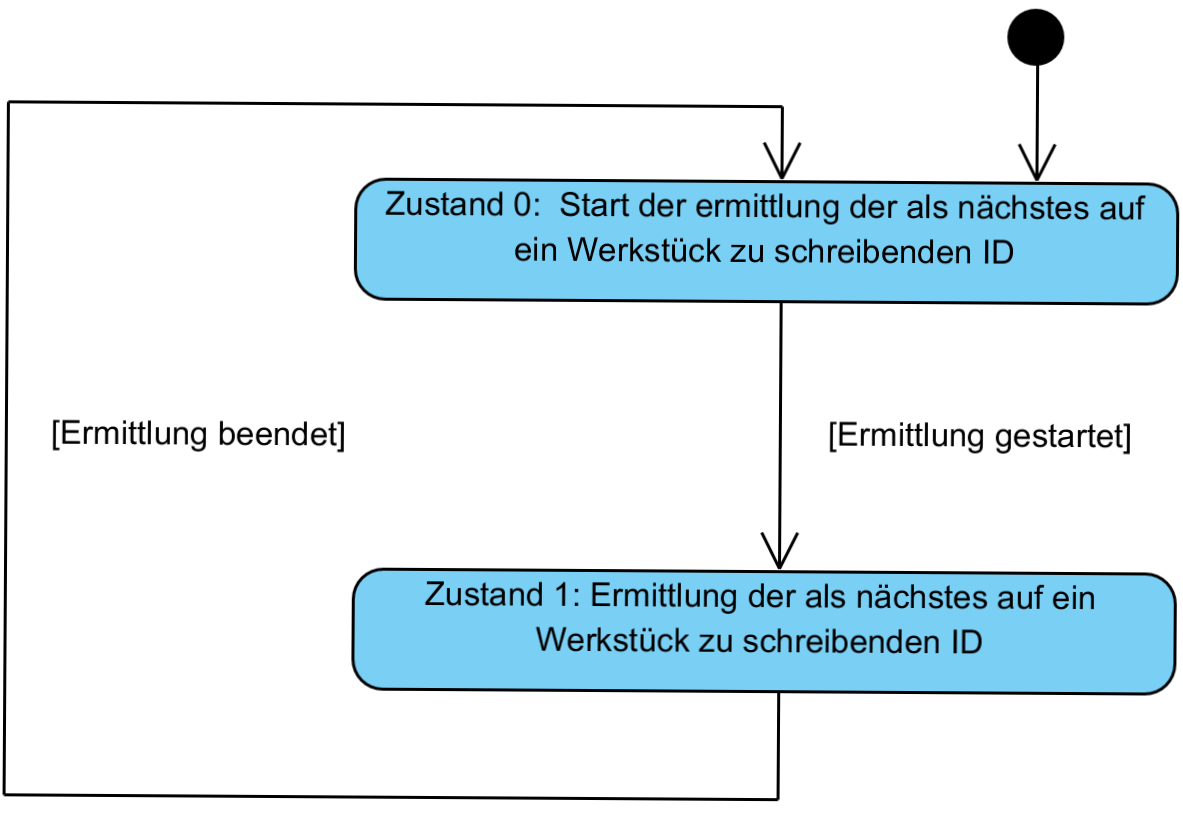
\includegraphics[width=0.7\linewidth]{Bilder/Zustandsdiagramme/taggen.png}
        \caption{UML-Zustandsdiagramm des FB Werkstueck\_taggen}
        \label{fig:FB_Werkstueck_taggen}
\end{figure}

\subsection{FB Timestamp\_anlegen}\label{kap:FB_Timestamp}
Der Funktionsbaustein \glqq Timestamp\_anlegen\grqq  ist zuständig für die Auswertung des RFID-Arrays, in dem die aktuell eingelesenen Werkstück id's gespeichert sind. Desweiteren Ermittelt der Funktionsbaustein alle für das anlegen des Timestamps erforderlichen Werte und schreibt mit Hilfe des Funktionsbausteins \glqq Datenbank\_Read\_Write\grqq  den Timestamp in die Datenbank. In der Abbildung \ref{fig:FB_Timestamp_anlegen} ist das Zustandsdiagramm des Funktionsbaustein dargestellt. 

\begin{figure}[h]
	    \centering
	    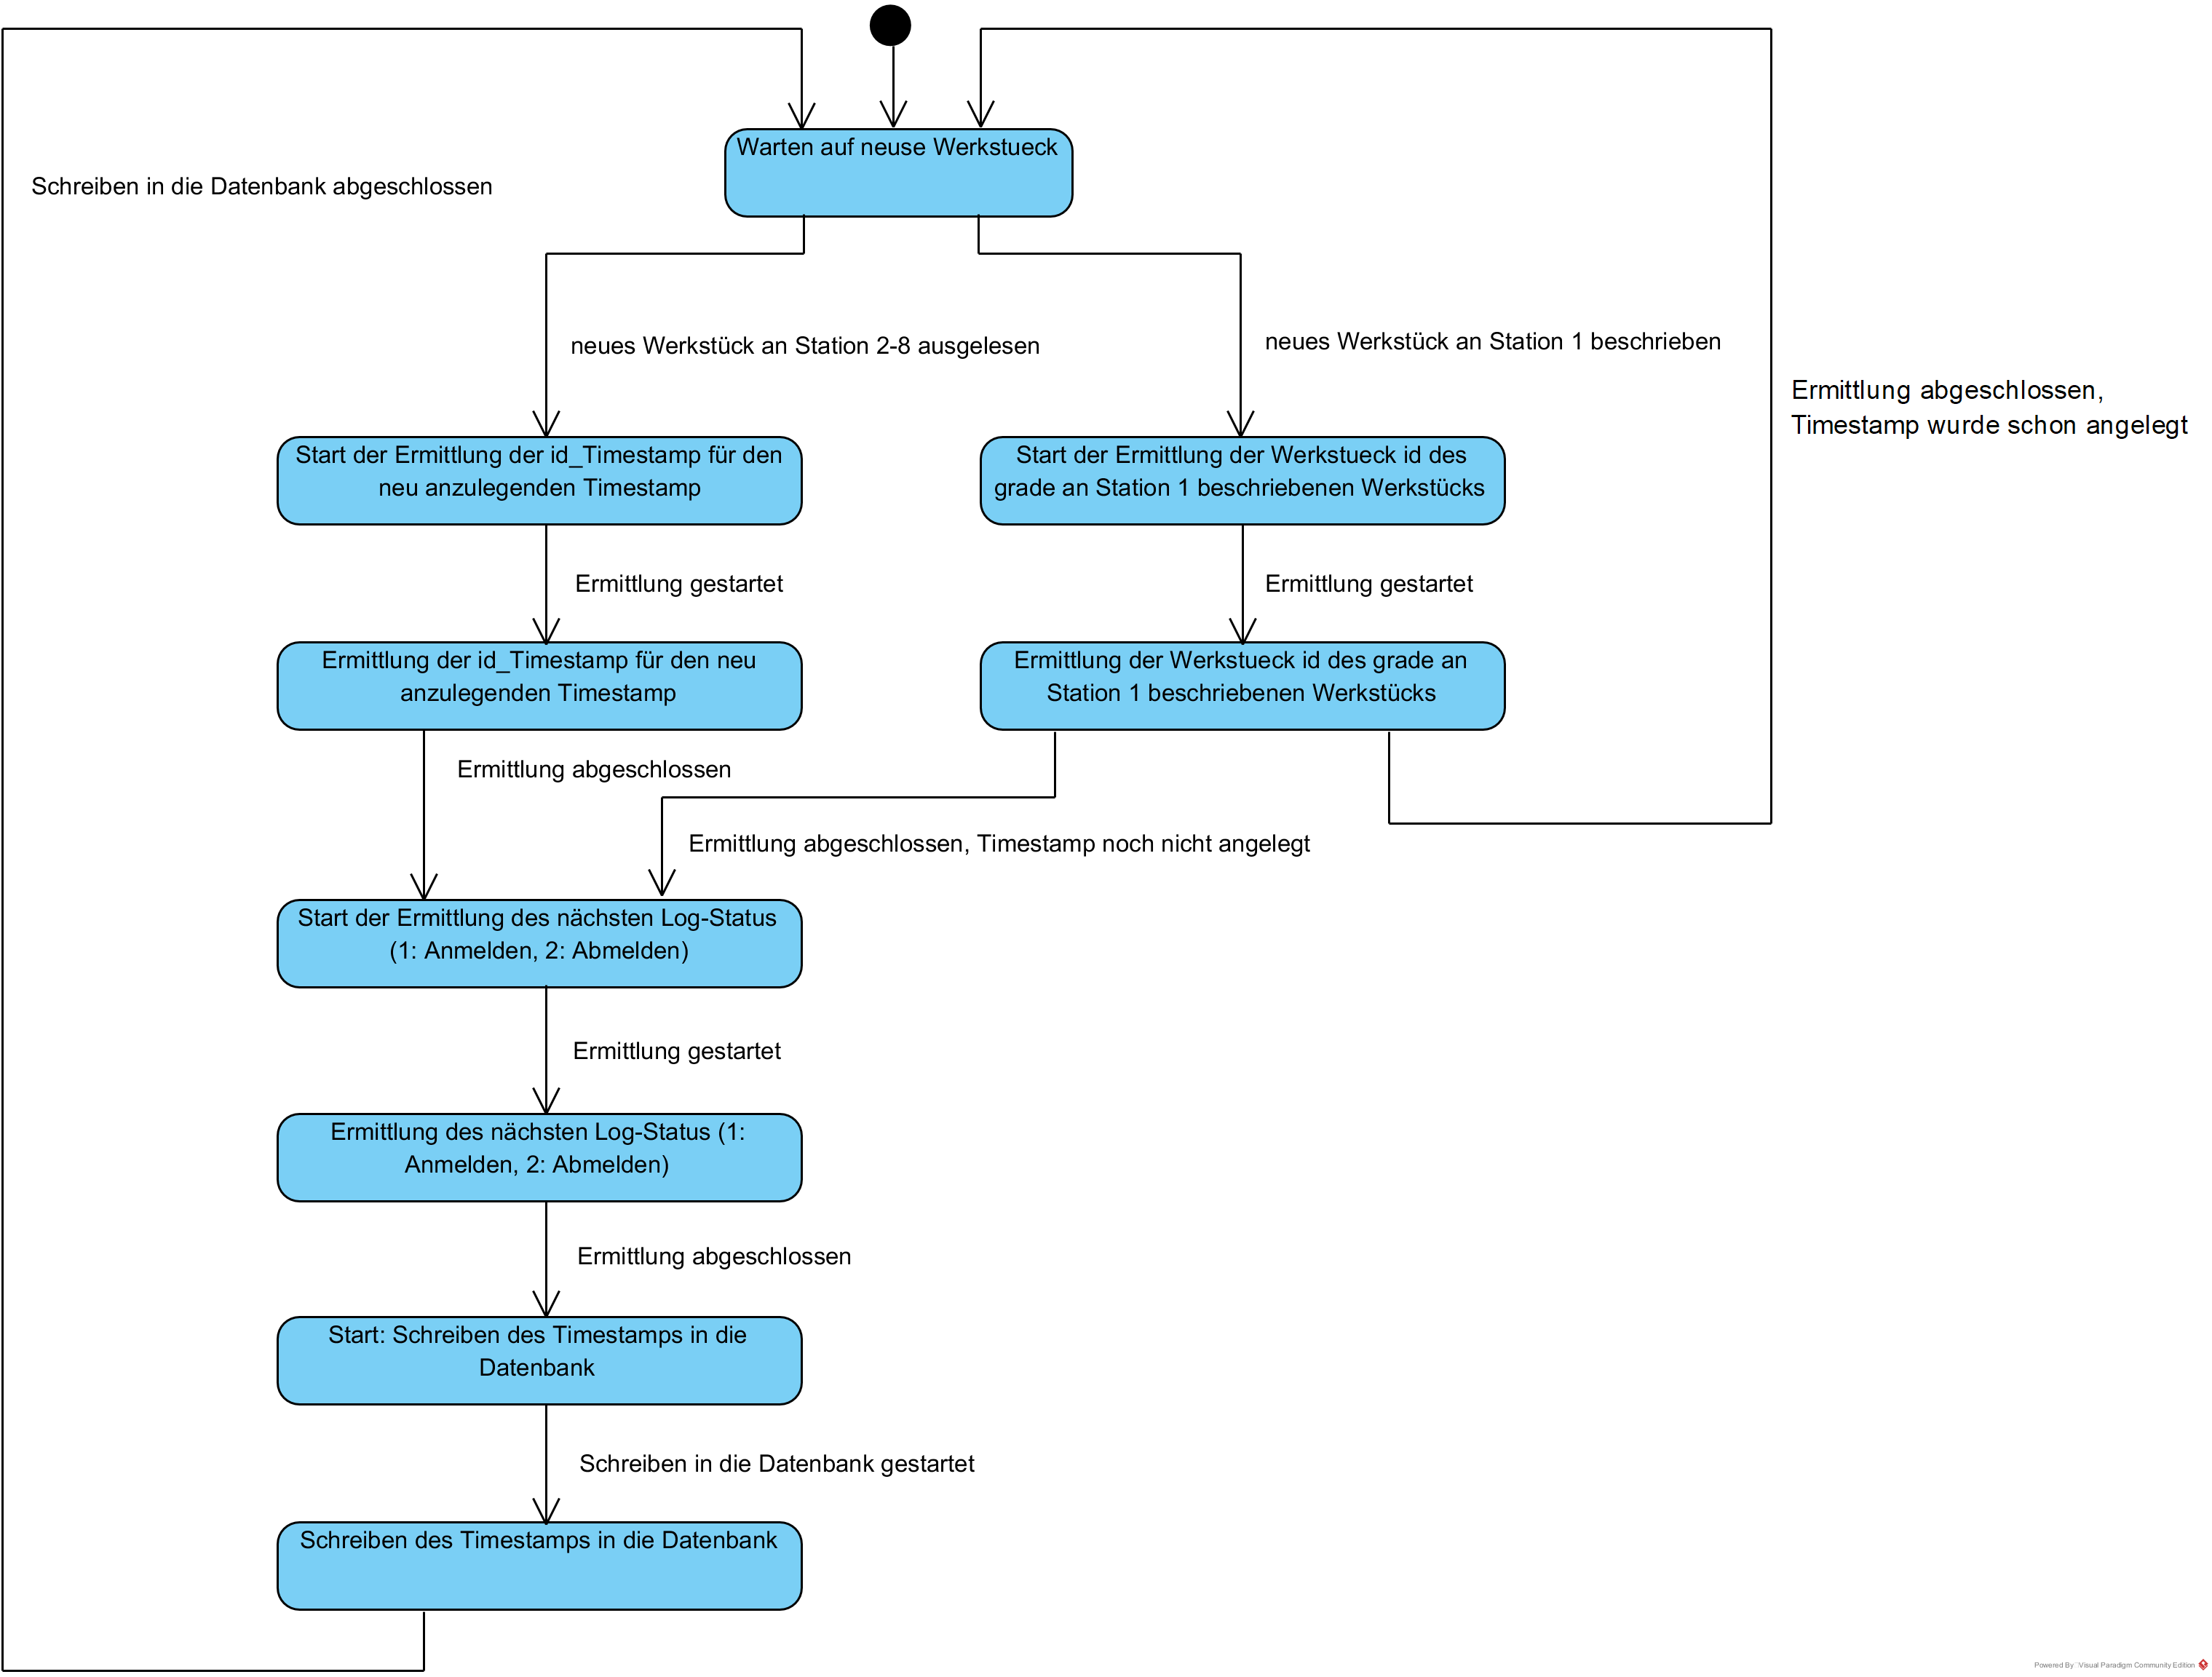
\includegraphics[width=1\linewidth]{Bilder/Zustandsdiagramme/Zustandsautomat_Timestamp.png}
        \caption{UML-Zustandsdiagramm des FB Timestamp\_anlegen}
        \label{fig:FB_Timestamp_anlegen}
\end{figure}

Zunächst wird im  Zustand 0 mit Hilfe der Funktion "`Su\-che\_neues\_Werk\-stueck"' nach einem neu unter den RFID-Lesekopf geschobenes Werkstück gesucht. Zu beginn wird allerdings zunächst geprüft ob an Station 10 ein Werkstück neue beschrieben wurde, dazu wird die globale Variable \glqq WRITE\_RFID\_DONE\grqq  ausgewertet und ggf. zurückgesetzt. Wurde kein Werkstück neu beschrieben wird überprüft ob sich seit dem letzten Aufruf der Funktion der Werte im RFID-Array geändert haben. Dazu wird ein Vergleich mit einer Kopie des Arrays aus dem letzten Aufruf durchgeführt. Wird eine Änderung erkannt, die sich  nicht auf 0 geändert hat, wird die Station an der die Änderung aufgetreten ist und die id des erkannten Werkstücks von der Funktion zurückgegeben. Ebenso wird die geänderte  Kopie des RFID-Arrays zurückgegeben.

Wurde ein Werkstück an Station 10 neu beschrieben, so muss zunächst mit einer Datenbank Abfrage aus der Tabelle \glqq taggen\grqq  die id des beschriebenen Werkstücks ermittelt werden. Dies geschieht im Zustand 2. Der Zustand 1 Startet die Ermittlung. Für einen Zugriff auf die Datenbank werden immer zwei Zustände benötigt, einer in dem die Abfrage gestartet wird und einer der die Abfrage ausführt und auf deren Ende wartet. 

Wurde die id des neu beschriebenen Werkstücks ermittelt, liegen genau die gleichen Informationen, nämlich die id des Werkstücks und die Station an der es erkannt wurde, wie bei einem Werkstück, dass neu unter einen Lesekopf der Stationen 2-8 geschoben wurde, vor. Für beide möglichen Fälle geht es weiter mit Zustand 3 und 4 wo die nächste frei id für den Timestamp aus der Datenbank ermittelt wird. Beim Übergang von Zustand 4 in Zustand 5 wird die aktuelle Zeit als Unix-Timestamp gespeichert. Anschließend wird im Zustand 5 und 6 der nächste Log-Status ermittelt. Der Log-Status beschreibt ob es sich um eine Anmeldung oder eine Abmeldung handelt. Zum ermitteln des Log-Status wird der letzte Eintrag für das jeweilige Werkstück in der Tabelle \glqq Timestamp\grqq  in der Datenbank ermittelt und der Status dementsprechend gesetzt. Besonders werden die Fälle an Station 10 und an Station 80 behandelt, da dort nur An- bzw. Abmeldungen möglich sind.

Nachdem nun die id des Werkstücks, die Station, die id des nächsten Timestamps, der nächste Log-Status und die aktuelle Zeit bekannt sind werden die Daten in den Zuständen 7 und 8 als Timestamp in der Datenbank abgelegt und zu Zustand 1 zurückgekehrt.

\subsection{FB Datenbank\_Read\_Write}\label{kap:FB_Datenbank_Read_Write}
Der Funktionsbaustein \glqq Datenbank\_Read\_Write\grqq  sorgt für einen geordneten Zugriff auf die Datenbank. Der eigentliche Zugriff auf die Datenbank findet in den vier Funktionsbausteinen \glqq SQL4Automation\_id\_Lesen\grqq , \glqq SQL4Automation\_nextLogStatus\-\_lesen\grqq , \glqq SQL4Automation\_RFID\_Werkstueck\_Lesen\grqq  und \glqq SQL4Automation\_Timestap\grqq \-statt. Da die Funktionsbausteine die selben globalen Variablen nutzen und mehrere Zyklen für einen Zugriff benötigen dürfen nicht mehrere der Funktionsbausteine gleichzeitig versuchen auf die Datenbank zuzugreifen. Da die Anfragen an die Datenbank von zwei verschiedenen Funktionsbausteinen aus erfolgt muss sichergestellt das die Anfragen nicht gleichzeitig erfolgt. Dafür wird dieser global instanzierte Funktionsbaustein genutzt. Wenn einer der Funktionsbausteine eine Anfrage stellen will wird geprüft ob diese Anfrage an der Reihe ist. Sollte die Anfrage nicht an der Reihe sein wartet der Funktionsbaustein bis die Anfrage an der Reihe ist und stellt jeden Zyklus erneut eine Anfrage. Der Funktionsbaustein \glqq Datenbank\_Read\_Write\grqq  prüft in dem Zustandsautomaten aus Abbildung \ref{fig:FB_Datenbank_Read_Write} ob eine Anfrage für den jeweiligen Datenbankzugriff vorliegt. Liegt keine Anfrage vor geht er zum nächsten Zustand wo auf eine Anfrage geprüft wird. Liegt einen Anfrage vor Startet er einen Datenbankzugriff und geht für die Dauer des Zugriffs in einen Zustand für die Ausführung der Anfrage. An die Anfragenden Funktionsbausteine meldet er zurück ob eine Datenbankzugriff gestartet wurde und ob der gestartete Zugriff abgeschlossen wurde.
\begin{figure}[h]
	    \centering
	    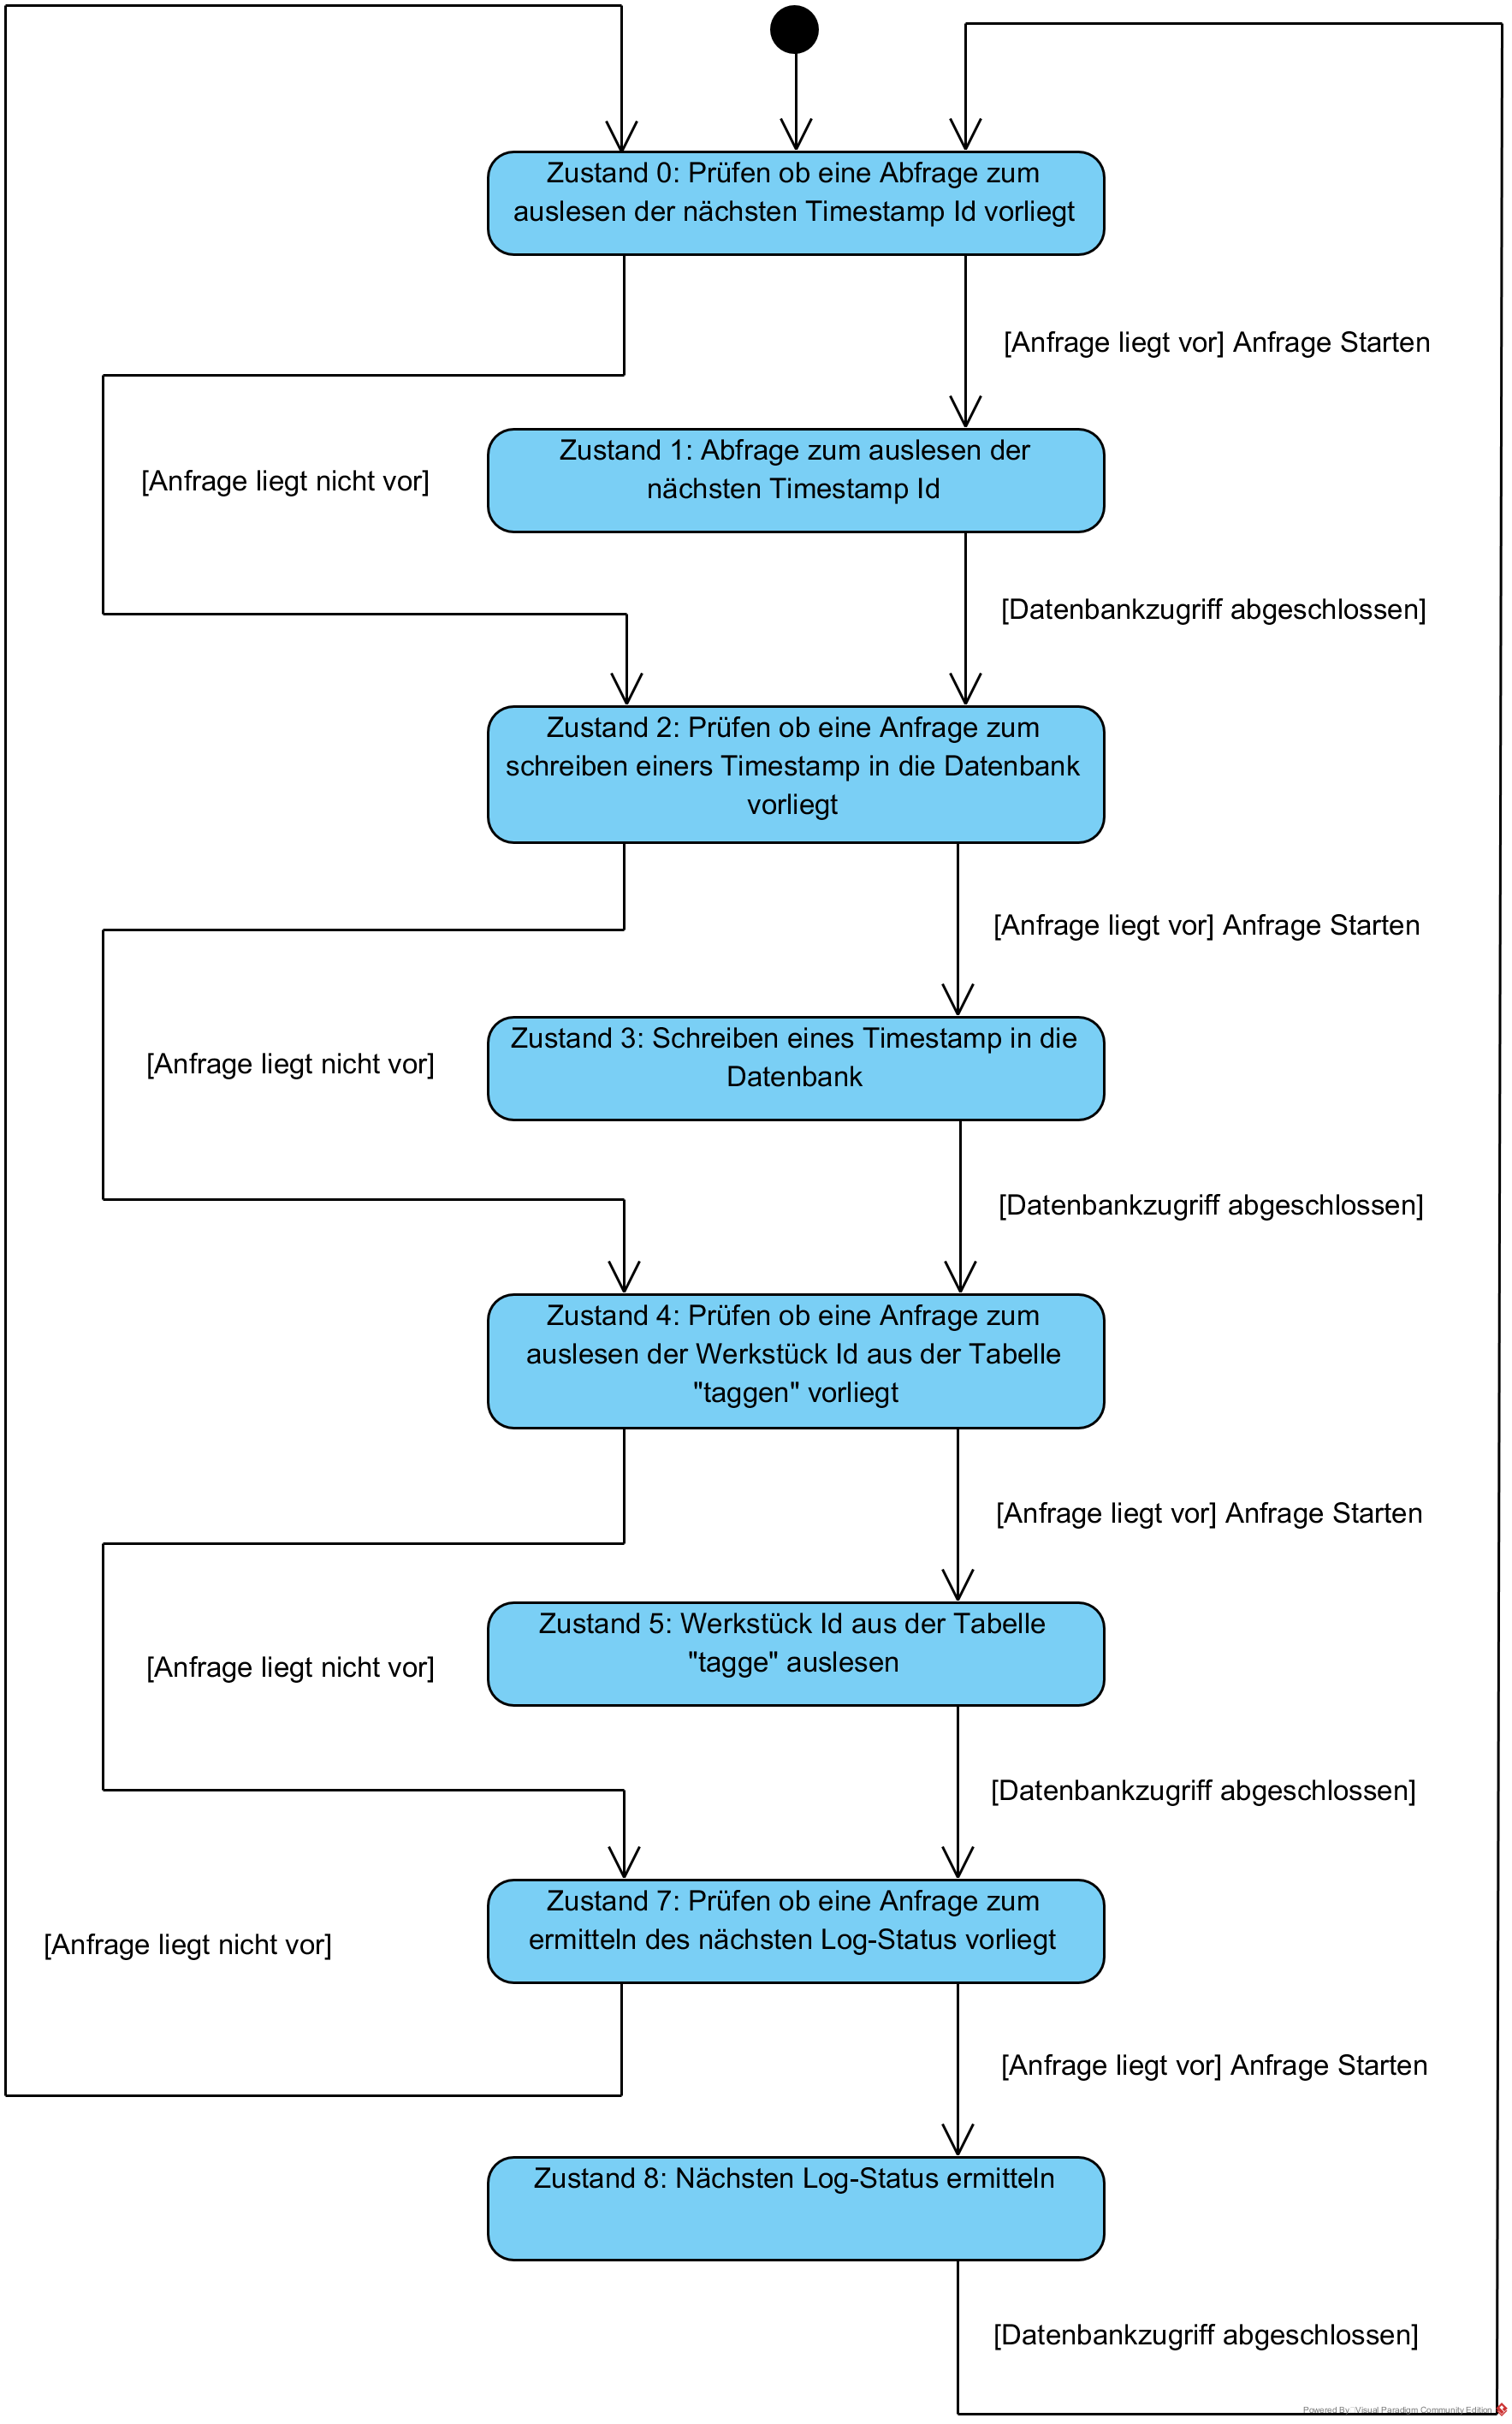
\includegraphics[width=0.8\linewidth]{Bilder/Zustandsdiagramme/Datenbank_Read_Write_State_Machine_Diagram.png}
        \caption{UML-Zustandsdiagramm des FB Datenbank\_Read\_Write}
        \label{fig:FB_Datenbank_Read_Write}
\end{figure}

\subsection{FB SQL4Automation}
Für jeden Zugriff auf die Datenbank ist ein seperater Funktionsbaustein zuständig. Aufgerufen werden die Funktionsbausteine durch den Funktionsbaustein "`Datenbank\_Read\_Write"´, der in Abschnitt \ref{kap:FB_Datenbank_Read_Write} beschrieben ist. Die Funktionsbausteine entsprechen in großen Teilen dem mit dem Staterkit zurverfügung gestellten Funktionsbaustein "`SQL4Automation\_2015"´. Angepasst wurde für die jeweiligen Funktionsbausteine der MySQL-Befehl zum Lesen oder Schreiben in der Datenbank. Desweiteren wurde bei Lesebefehlen ein zusätzlicher Rückgabewert für das Ergebnis der Abfrage und die entsprechende Konvertierung des Rückgabe-Strings der Datenbank in den richtigen Datentyp hinzugefügt. Ebenso wurde eine Rückgabevariable hinzugefügt die zurückmeldet ob die Anfrage an die Datenbank abgeschlossen ist. Wie schon in Kapitel \ref{kap:FB_Datenbank_Read_Write} beschrieben nutzen alle Funktionsbausteine, die den Zugriff auf die Datenbank durchführen die selben globalen Variablen. Da ein Zugriff mehrere Zyklen dauert ist sicherzustellen das nicht zwei Funktionsbausteine zur selben Zeit eine Anfrage an die Datenbank stellen. 

\subsection{Systemzeit Einstellen}
Da die Systemzeit nach jedem Start der Soft-SPS auf den default-Wert 1. Januar 1970 0:00:00 Uhr gesetzt wird und das manuelle einstellen der Systemzeit bei jedem Neustart der Soft-SPS Beziehungsweise des aufgespielten CODESYS-Programms ungenau und aufwendig ist wird die aktuelle Mitteleuropäische Zeit zu beginn des Programms automatisch ermittelt. Zur Ermittlung der Zeit für die Timestamps wird der Funktionsbaustein "`RTC"´ genutzt. Dieser wird zu Programmbegin im Funktionsbaustein "`Timestamp\_anlegen"´ einmal initialisiert. Für die Initialisierung wird die aktuelle Zeit im Datentype DT benötigt. Die aktuelle Zeit wird zu Programmbegin in der Main über die Datenbank ermittelt. 

Wie in Abbildung \ref{fig:ER-Diagramm_Worbenche} zu sehen gibt es in der Datenbank eine Tabelle mit dem Namen Zeit, diese Tabelle hat nur eine Zeile in der es einmal den Primärschlüssel "`id\_Zeit"` und das Feld "`aktuelle\_Zeit"´gibt. Bei Start des Programms wird in der Main zunächst der Funktionsbaustein "`SQL4Automation\_aktuelle\_Zeit"´ aufgerufen, dabei handelt es sich um den einzigen Funktionsbaustein der auf die Datenbank zugreift und nicht über den Funktionsbaustein "`Datenbank\_Read\_Write"´ aufgerufen wird. Da das ermitteln der aktuellen Zeit erst abgeschlossen sein muss bevor der restliche Programmteil startet besteht keine Gefahr eines gleichzeitigen Zugriffs.
Der Funktionsbaustein "`SQL4Automation\_aktuelle\_Zeit"´ führt die zwei in den Listings \ref{lst:MySQL_Zeit1} und \ref{lst:MySQL_Zeit2} dokumentierten SQL-Befehle aus.
Der Befehl aus Listing \ref{lst:MySQL_Zeit1} aktualisiert die Zeit im Feld "`aktuelle\_Zeit"´ in der Datenbank. Mit dem Befehl in Listing \ref{lst:MySQL_Zeit2} wird diese abgefragt.
\lstset{ 
    keywordstyle        =\bfseries\ttfamily\color{blue},
    basicstyle          =\scriptsize\ttfamily, 
    emphstyle           =\color{red},
    numbers             =left,
    xleftmargin         =15pt,
    backgroundcolor     =\color{lightgray},
    showstringspaces    =false,
    language            =SQL
    }	 

\begin{lstlisting}[caption={MySQL-Befehl: Zeit aktualisieren}
       \label{lst:MySQL_Zeit1},
       captionpos=t] 
UPDATE vpj.Zeit
SET
    aktuelle_Zeit = NOW()
WHERE
    id_ZEIT = 1;
\end{lstlisting}

\lstset{ 
    keywordstyle        =\bfseries\ttfamily\color{blue},
    basicstyle          =\scriptsize\ttfamily, 
    emphstyle           =\color{red},
    numbers             =left,
    xleftmargin         =15pt,
    backgroundcolor     =\color{lightgray},
    showstringspaces    =false,
    language            =SQL
    }	 

\begin{lstlisting}[caption={MySQL-Befehl: Zeit abfragen}
       \label{lst:MySQL_Zeit2},
       captionpos=t] 
SELECT
    aktuelle_Zeit
FROM
    vpj.Zeit
WHERE
    id_ZEIT = 1;
\end{lstlisting}

Mit Hilfe von String-Operationen wird der zurückgelieferte String so umgebaut das er mit Hilfe eines Cast vom Datentype String in den Datentype DT (Date and Time) umgewandelt werden kann. 